\documentclass[twocolumn]{article}
\usepackage{usenix-2020-09}
\usepackage[backend=biber]{biblatex}
\usepackage{biblatex}
\usepackage{inconsolata}
\usepackage{minted}
\definecolor{bg}{rgb}{0.97,0.97,0.97}
\usepackage{graphicx}
\bibliography{ref}

\begin{document}
\date{}
\title{\Large \bf AMD Confidential Computing Technologies Evaluation Report}
\author{{\rm Roberto Castellotti}\\TU Munich \and {\rm Masnori Misono}\\TU Munich}
\maketitle
% https://github.com/TUM-DSE/research-work-info/tree/master/thesis-report
TODO:
\begin{itemize}
    \item change kernel version
    \item update my repository to use the same scripts I am using in tum-dse/cvm\_evaluate
    \item license for repository?
    \item bios configuration
    \item kernel isse masa solved, should we mention it?
\end{itemize}

\begin{abstract}
    Confidential Computing is a topic that started to become relevant in the last 20 years. In the last two decades the way software is shipped to production changed radically, almost everyone now uses cloud providers (Google Cloud Platform, Amazon Web Services, Microsoft Azure, etc.). This leads to customers running their code on machines they don't own. It is logic customers want to be sure no one can access their disks, memory or CPU registers, not other customers running virtual machines on the same hardware, nor whoever is controlling the hypervisor be it  the cloud vendor  or, in worst case scenarios, malign actors who compromised the physical machines. Encryption at rest (designed to prevent the attacker from accessing the unencrypted data by ensuring the data is encrypted when on disk from Microsoft, cite properly) has been around for a long time, and is currently supported by all major providers \cite{aws-enc}, \cite{gcp-enc}, \cite{azure-enc} but this leaves a big part of daily computing unencrypted, namely RAM and CPU registers, to tackle this issue major chip producers started to develop a technlogy to enable "confidential computing", 
    namely AMD Secure Encrypted Virtualization (SEV) \cite{memory-encryption}, Intel Trusted Domain Extensions (TDX) \cite{tdx} and Arm Confidential Compute Architecture (CCA) \cite{cca}

    We report a preliminary performance evaluation of AMD SEV (Secure Environment Virtualization) technologies.
    We run our experiments on ryan, using a patched version of QEMU from AMD. We use QEMU/KVM as a hypervisor. We assign the guest the same amount of CPUs (16) and 16G of memory. Further details about our environment can be found in section \ref{sec:environment}

\end{abstract}


\begin{table*}
    \centering
    \label{tab:experiment-environment}
    \begin{tabular}{l|l}
        \hline
        Host CPU      & \texttt{AMD EPYC 7713P 64-Cores}                                            \\
        Host Memory   & \texttt{HMAA8GR7AJR4N-XN (Hynix) 3200MHz 64 GB $\times$ 8 (512GB)}          \\
        Host Kernel   & \texttt{6.3.0-rc2 \#1-NixOS SMP PREEMPT\_DYNAMIC (NixOS 23.05)}             \\
        QEMU          & \texttt{8.0.0 (AMD) (patched)}                                              \\
        OVMF          & \texttt{Stable 202211 (patched)}                                            \\
        Guest vCPUs   & \texttt{16}                                                                 \\
        Guest Memory  & \texttt{16GB}                                                               \\
        Guest Kernel  & \texttt{5.19.0-41-generic \#42-Ubuntu SMP PREEMPT\_DYNAMIC (Ubuntu 22.10 )} \\ 
        \hline
    \end{tabular}
    \caption{Experiment environment}
\end{table*}

\section{AMD Secure Memory Encryption (SME)}
AMD Secure Memory Encryption (SME) is the basic building block for the more sophisticated technologies we'll cover later, so it is imperative we understand how it works. In a machine with SME enabled memory operations are performed via dedicated hardware, an entirely different chip on die. AMD EPYC™ introduced two hardware security components:
\begin{description}
    \item [AES-128 hardware encryption engine] embedded in memory controller, makes sure data to main memory is encrypted during write opeartions and decrypted during read operations, this memory controller is inside the EPYC SOC, so memory lines leaving the soc are encrypted
    \item [AMD Secure Processor] a small processor providing cryptographic functionality for secure key generation and key management
\end{description}

\begin{figure}
    \centering
    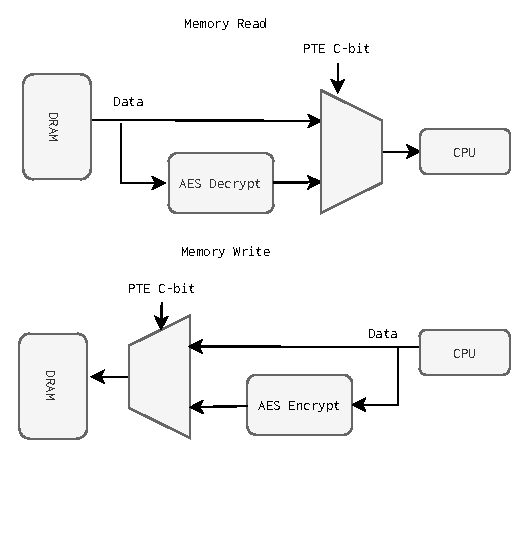
\includegraphics[scale=0.25]{img/read-write.png}
    \caption{Memory Encryption Behaviour, from \cite{memory-encryption}}
\end{figure}

The key used to encyrpt and decrypt memory is generated securely by the AMD Secure-Processor (SMD-SP), a 32 bit microcontroller and it is not accesible by software running on the main CPU, furthermore SME does not require software running on main CPU to partecipate in Key Management making the enclave more secure.

The C-bit is a bit present in any memory page and indicates whether the current page is to be encrypted, it can be retrieved toghether with some additional infos by running the \texttt{cpuid} command to inspect leaf \texttt{0x8000001F}, as specified by AMD Reference Manual (do i need to cite it?):

\begin{minted}[bgcolor=bg,fontsize=\footnotesize]{bash}
$ cpuid -1 -l 0x8000001F
CPU:
AMD Secure Encryption (0x8000001f):
    SME: secure memory encryption support    = true
    SEV: secure encrypted virtualize support = true
    VM page flush MSR support                = true
    SEV-ES: SEV encrypted state support      = true
    SEV-SNP: SEV secure nested paging        = true
    VMPL: VM permission levels               = true
    Secure TSC supported                     = true
    virtual TSC_AUX supported                = false
    hardware cache coher across enc domains  = true
    SEV guest exec only from 64-bit host     = true
    restricted injection                     = true
    alternate injection                      = true
    full debug state swap for SEV-ES guests  = true
    disallowing IBS use by host              = true
    VTE: SEV virtual transparent encryption  = true
    VMSA register protection                 = true
    encryption bit position in PTE           = 0x33 (51)
    physical address space width reduction   = 0x5 (5)    
    number of VM permission levels           = 0x4 (4)
    number of SEV-enabled guests supported   = 0x1fd (509)
    minimum SEV guest ASID                   = 0x80 (128)
\end{minted}
    
SME is a very powerful mechanism to provide memory encryption, but it requires support from the Operating System/Hypervisor, \textbf{Transparent SME (TSME)} is a solution to encrypt every memory page regardeless of the C-bit, as the name suggests this technology provides encryption without further modification to OS/HV, this may be crucial because Operating System developers don't have to support it and older operating systems can be run with TSME.

We now switch our focus to AMD SEV, a technology powered by AMD SME that enables Confidential Computing for virtual machines.

\section{AMD Secure Encrypyted Virtualization (SEV)}

AMD SEV is an attempt to make virtual machines more secure to use by encrypting data to and from a virtual machine, and enables a new security model protecting code from higher privileged resources, such as hypervisors or some privileged code running on the phyisical machine hosting the virtual machines. In this context, as mentioned before, we should never trust the hypervisor since it may be compromised or acting maliciously by default.

\begin{figure}
    \centering
    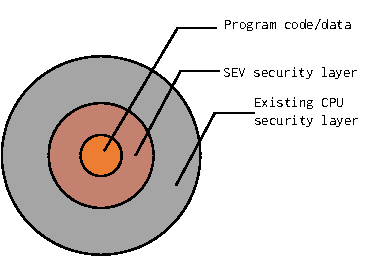
\includegraphics[scale=0.25]{img/security-layers.png}
    \caption{SEV security layers, from \cite{memory-encryption}}
\end{figure}

SEV is an extension to the AMD-V architecture, when SEV is enabled SEV machines tag data with VM ASID (an unique identifier for that specific machine), this tag is used inside the SOC and prevents external entities to access it, when data leaves the chip we have no such problem because it is encrypted using the previously exchanged AES-128 bit key. The aforementioned expedients provide strong cryptography isolation between VMs run by the same hypervisor and between VMs and the hypervisor by itself. SEV guests can choose which pages to encrypt, this is handled setting the c-bit as mentioned before for SME. Only pages meant fot oustide communcations are considered shared and thus not encrypted.

\section{AMD Secure Encrypted Virtualization-Encrypted State (SEV-ES)}

Up until now we only discussed encryption for memory, but a crucial portion of the system we want to protect are CPU registers, AMD SEV-ES encrypts all CPU register contents when a VM stops running. What this means is a malevolent actor is not able to read CPU's register contents when the machine is shutdown no matter the privilege level he acquired before, CPU register's state is saved and encrypted when the machine is shutdown.

Protecting CPU register may be a daunting task because sometimes an Hypervisor may need to access VM CPU's register to provide services such as device emulation. These accesses must be protected, ES technlogy allows the guest VM to decide which registers are encrypted, in the same vein a machine can choose which memory pages are to be encrypted via the C-bit.

SEV-ES introuduces a single atomic hardware instruction: \texttt{VMRUN}, when this intruction is executed for a guest the CPU loads all registers, when the VM stops runnning (\texttt{VMEXIT}), register's state is saved automatically to  back to memory. These instructions are atomic because we need to be sure no one can sneak into this process and alter it, ES guarantees in this way it is impossible to leak memory.

Whenever hardware saves register it encrypts them with the very same AES-128 key we mentioned before, furthermore the CPU computes an integrity-check value and saves it into memory not accessible by the CPU, on next \texttt{VMRUN} instruction this will be checked to ensure nobody tried to tamper register's state. For further information about external communication consult the whitepaper (CITE) and AMD reference manual chapter 15 (HOW TO CITE THE SPECIFIC CHAPTER?).

Similarly to AMD-SEV AMD-ES is completely transparent to application code, only the guest VM and the Hypervisor need to implement these specific features.

\section{AMD Secure Encrypted Virtualization-Secure Nested Paging (SEV-SNP)}

After the introduction of AMD-SEV an AMD-ES AMD decided to introduce the next generation of SEV called Secure Nested Paging (SEV-SNP), this technlogy build on top of the aforementioned technlogies and extends them further to implement strong memory integrity protection to prevent Hypervisor based attacks, such as \textbf{replay attacks} and \textbf{memory remapping}, \textbf{data corruction} and \textbf{memory aliasing}

\begin{description}
    \item[replay attacks] a malicious actor captures a state at a certain moment and modifies memory succesfully with those values
    \item[data corruption]  even though an attacker cannot read a memory he can simply corrupt the memory to trick the machine into unpredicted behaviour
    \item[memory aliasing]  an external actor may map a memory page to multiple physical pages
    \item[memory remapping]  the intruder maps a page to a different physical page
\end{description}

These attacks are a problem because a running program has no notion of memory integrity, they could end up in a state that was not originally considered by the developers and this may lead to huge security issues.

The basic principle of \textbf{SEV-SNP} integrity is that if a VM is able to read a private (encrypted) page of memory, it must always read the value it last wrote. (cite) What this means is the VM should be able to throw an exception if the memory a process is trying to access was tampered by external actors.

\subsection*{Threat Model}
In this computing model we consider:

\begin{itemize}
    \item \textbf{AMD System-On-Chip (SOC) hardware}, \textbf{AMD Secure Processor (AMD-SP)} and the \textbf{VM} are fully trusted, to this extend the VM should enable Full Disk Encryption (FDE) at rest, such as LUKS (cite), major cloud providers have been supporting FDE for long time:  https://cloud.google.com/docs/security/encryption/default-encryption
    \item \textbf{BIOS} on the host system, the \textbf{Hypervisor}, \textbf{device drivers} and \textbf{other VMS} are fully untrusted, this means the threat model assumes they are malicious and may conspire to compromise the security of our Confidential Virtual Machine.
\end{itemize}

The way SEV-SNP ensures protection against the attacks we mentioned before is by introudcing a new data structure, a \textbf{Reverse Map Table (RMP)} that tracks owners of memory pages, in this way we can enforce that only the owner of a certain memory page can alter it. A page can be owned by the VM, the Hypervisor or by the AMD Secure Processor. The RMP is used in conjunction with standard x86 page tables mechanisms to enforce memory restrictions and page access rights. RMP fixes replay, remapping and data corruction attacks. 

RMP checks are introduced for write operations on memory, however external (Hypervisor) read accesses do not require them because we have AES encryption protecting our memory.

To prevent memory remapping a technique called \textbf{Page Validation} is introduced.
Inside each RMP entry there is a Validated bit, pages assigned to guests that have no validated bit set are not usable by the Hypervisor, the guest can only use the page after setting the validated bit through a \texttt{PVALIDATE} instruction. The VM will make sure that it is not possible to validate a SPA (system phyiscal address) corresponding to a GPA (Guest Physical Address) more than once.
 
More details are discussed in the introductory whitepaper \cite{sev-snp}

We now introduced every part of AMD's effort to popularize Confidential Computing, now we will proceed by giving instructions to start such machines using QEMU/KVM and we will run some benchmarks to measure how these technlogies impact performance.


\section{Environment}

\begin{itemize}
    \item mention we need uefi and this is why we have ovmf
\end{itemize}
\label{sec:environment}
OVMF is a project maintanied by TianoCore aiming to enable UEFI support for virtual machines, it is based on EDK 2, we will use OVMF to generate the executable firmware and the non-volatile variable store, it is important to create a vm-specific cody of OVMF\_vars.fd because the variable store should be private for every virtual machine

QEMU is a generic open source machine emulator and virtualizer, we will use QEMU toghether with KVM, the Kernel Virtual machine to virtualize our machines.

\section{Benchmarks}

We are running three distinct kinds of benchmarks: Compilation, Memory Benchmarks and I/O benchmarks to evaluate whether using the aforementioned confidential technology incurs in some overhead. To run the benchmarks we are using rcastellotti/tinyben \cite{tinyben}, an experimental benchmarking tool aimed to replace the popular Phoronix Test Suite \cite{pts} benchmarking suite.

\begin{description}
    \item[Compilation Benchmarks] We are using compilation as an all-around benchmark because it is a "real world" benchmark. We are compiling some popular opensource projects like \href{https://github.com/godotengine/godot}{Godot Game Engine}, \href{https://github.com/imagemagick/imagemagick}{ImageMagick} (using gcc), \href{https://git.kernel.org/pub/scm/linux/kernel/git/torvalds/linux.git}{Linux} (defconfig), the entire \href{https://github.com/llvm/llvm-project}{LLVM Project} (using ninja) and measuring how long does it take to complete the compilation process.
    \item[Memory Benchmarks] To bechmark memory we are using ssvb/tinymembench \cite{tinymembench}, a tool to measure memory throughput and latency, we are mainly interested in bandwidth for the \texttt{MEMCPY} and \texttt{MEMSET} operations
    \item[I/O Benchmarks] To measure I/O performance we are running two different benchmarks, first we are performing 2500 sqlite insertions in a table, then we are running redis-benchmark, a tool shipped toghether with redis. We are interested in Requests per Second and latency for the main operations. 
\end{description}

\begin{table*}
    \centering
    \label{tab:tinyben-results}
    \begin{tabular}{l|r|r}
    \textbf{benchmark}                        & \textbf{SEV-SNP} & \textbf{NOSEV} \\
    \hline
    Godot Game Engine compilation (LIB)       &  410 sec         & 395 sec        \\
    ImageMagick compilation (gcc) (LIB)       &  70 sec          & 69 sec         \\
    Linux compilation (defconfig) (LIB)       &  329 sec         & 322 sec        \\
    LLVM Project compilation (ninja) (LIB)    &  774 sec         & 733 sec        \\
    Sqlite 2500 insertions (LIB)              &  4.106 sec       & 4.31 sec       \\
    ssvb/tinymembench MEMCPY (HIB)            &  22727.0 MB/s    & 23628.2 MB/s   \\
    ssvb/tinymembench MEMSET (HIB)            &  33170.8 MB/s    & 36367.7 MB/s   \\
    redis-benchmark SET RPS (HIB)             &  91911.76        & 110864.74      \\
    redis-benchmark SET average latency (LIB) &  0.283 msec      & 0.234 msec     \\
    redis-benchmark GET RPS (HIB)             &  94339.62        & 110987.79      \\
    redis-benchmark GET average latency (LIB) &  0.275 msec	     & 0.233 msec     \\
    \end{tabular}
    \caption{Comparing benchmark results run on two QEMU vms (16 vCPUs, 16GB ram, virtio-scsi storage). HIB and LIB mean respectively "Higher is Better" and "Lower is Better", RPS stands for "Requests Per Second"} 
\end{table*}

As we can see in table \ref{tab:tinyben-results} the overhead introduced by the usage of Confidential Computing technology across the three categories of benchmarks is generally mild, and negligible in certain cases (ImageMagick compilation and Sqlite benchmark), further investigation tweaking the amount of resources available to each machine is necessary to correcly esteem the exact performance degradation values.

We ran some additional benchmarks regarding the different storage virtualization techniques, more specifically we tested \textbf{virtio-scsi}, 
\textbf{virtio-blk} and \textbf{nvme} technologies. Virtio is the main platform for IO virtualization in KVM, essentially it provides a common framework for hypervisors to do IO virtualization.

\begin{description}
    \item[nvme] is the userspace NVMe driver that enables virtual machines to interact with NVMe devices
    \item[virtio-blk] devices are very simple block devices, the frontend driver reads and writes by appending commands to the virtualization queue so that the Backedn driver can process them on the host.
    \item[virtio-scsi] aims to overcome some limitations introduced by virtio-blk, support more devices per guest (one PCI device per disk is not a limiting factor anymore) and supports technlogies like multiqueueing while keeping the performances of virtio-blk, additionally virtio-scsi provides a passthrough technlogy to present physical storage devices directly to guests
\end{description}

We perform some measurements using the fio \cite{fio} benchmarking tool, we use the same measurements used in \cite{spool} to evaluate: bandwidth, average latency and IOPS, we use the \texttt{--direct=1} flag to use unbuffered I/O.

\begin{figure}
    \centering
    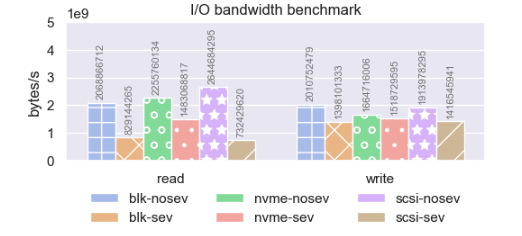
\includegraphics[width=1\columnwidth]{img/bw.png}
    \caption{Storage Bandwidth Benchmarks}
\end{figure}
\begin{figure}
    \centering
    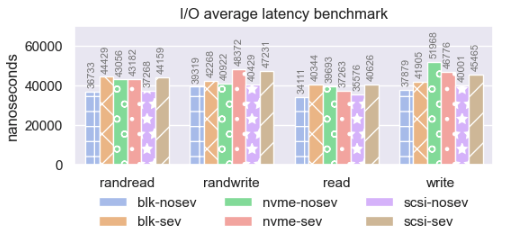
\includegraphics[width=1\columnwidth]{img/al.png}
    \caption{Average Latency}
\end{figure}
\begin{figure}
    \centering
    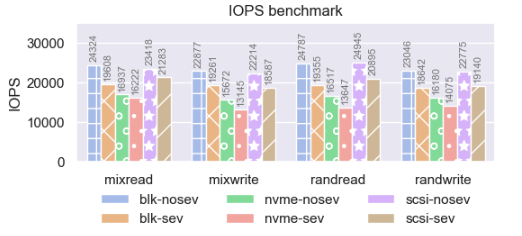
\includegraphics[width=1\columnwidth]{img/iops.png}
    \caption{I/O operations per second benchmark}
\end{figure}


\section{Future Work}
in SEV-ES it seems like VMRUN and VMEXIT need to perform some additional tasks, can we benchmark this in some way?
- https://jcadden.medium.com/confidential-computing-with-kubernetes-sev-guest-protection-for-kata-containers-8f29f0a3a2d7

item sev tio 
explore coco (chrome bookmarks)
item sev svsm

\printbibliography
\appendix
\section*{Appendix}
\section{A simple attack to demo Confidential Computing}
Let's demo a very simple attack, first of all we start two machines, \textit{sev} and \textit{nosev}, the former has SEV-SNP enabled, as we can check:

\begin{minted}[bgcolor=bg,fontsize=\footnotesize]{bash}
sev:~$ sudo dmesg | grep SEV
Memory Encryption Features active: AMD SEV SEV-ES SEV-SNP
SEV: Using SNP CPUID table, 31 entries present.
SEV: SNP guest platform device initialized.
\end{minted}

We will write something into a file and cat it in order to load the data in memory

\begin{minted}[bgcolor=bg,fontsize=\footnotesize]{bash}
sev:~$ echo "hi from SEV!" > sev.txt
sev:~$ cat sev.txt
hi from SEV!
\end{minted}

\begin{minted}[bgcolor=bg,fontsize=\footnotesize]{bash}
nosev:~$ echo "hi from NOSEV!" > nosev.txt
nosev:~$ cat nosev.txt
hi from NOSEV!
\end{minted}

Now we can dump the memory for the processes using \texttt{gcore}

\begin{minted}[bgcolor=bg,fontsize=\footnotesize]{bash}
h:~$ sudo gcore -o mem-dump <SEV_PID>
h:~$ grep -rnw mem-dump.<SEV_PID> -e "hi from SEV!"
h:~$
\end{minted}

\begin{minted}[bgcolor=bg,fontsize=\footnotesize]{bash}
h:~$ sudo gcore -o mem-dump <NOSEV_PID>
h:~$ grep -rnw mem-dump.<NOSEV_PID> -e "hi from NOSEV!"
grep: mem-dump.<NOSEV_PID>: binary file matches
\end{minted}

From the host machine we are able to see nosev's machine memory while this is not possible with SEV enabled.

\end{document}